
\hypertarget{menu_insert}{}
\section{Insert}
\index{insert menu}

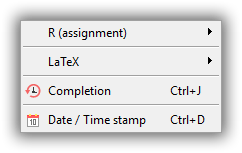
\includegraphics[scale=0.50]{./res/menu_insert.png}\\

\begin{scriptsize}
  \begin{tabularx}{\textwidth}{>{\hsize=0.3\hsize}X>{\hsize=0.7\hsize}X}\\
    \hline
    \textbf{Option} & \textbf{Description} \\
    \hline
    R (assignment) & \textit{\href{\#menu\_insert\_r}{See options ...}} \\
    \LaTeX & \textit{\href{\#menu\_insert\_latex}{See options ...}} \\
    \hdashline[1pt/1pt]
    Date / Time stamp & Inserts the current system time and date \\
    Snippet insert (trigger context) & Replaces the trigger with the corresponding block of text (snippet) \\
    \hline
  \end{tabularx}
\end{scriptsize}


\hypertarget{menu_insert_r}{}
\subsection{R (assignment)}
\index{insert menu!R}

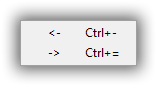
\includegraphics[scale=0.50]{./res/menu_insert_r_assignment.png}\\

\begin{scriptsize}
  \begin{tabularx}{\textwidth}{>{\hsize=0.3\hsize}X>{\hsize=0.7\hsize}X}\\
    \hline
    \textbf{Option} & \textbf{Description} \\
    \hline
    <- & Insert left assignment \\
    -> & Insert right assignment \\
    \hline
  \end{tabularx}
\end{scriptsize}


\hypertarget{menu_insert_latex}{}
\subsection{Latex}
\index{insert menu!LaTeX}

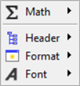
\includegraphics[scale=0.50]{./res/menu_insert_latex.png}\\

\begin{scriptsize}
  \begin{tabularx}{\textwidth}{>{\hsize=0.3\hsize}X>{\hsize=0.7\hsize}X}\\
    \hline
    \textbf{Option} & \textbf{Description} \\
    \hline
    Math & \textit{\href{\#menu\_insert\_latex\_math}{See options ...}} \\
    \hdashline[1pt/1pt]
    Header & \textit{\href{\#menu\_insert\_latex\_header}{See options ...}} \\
    Format & \textit{\href{\#menu\_insert\_latex\_format}{See options ...}} \\
    Font & \textit{\href{\#menu\_insert\_latex\_font}{See options ...}} \\
    \hline
  \end{tabularx}
\end{scriptsize}


\hypertarget{menu_insert_latex_math}{}
\subsubsection{Math:}\\
\index{insert menu!LaTeX math}

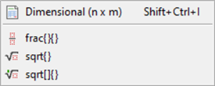
\includegraphics[scale=0.50]{./res/menu_insert_latex_math.png}\\

\begin{scriptsize}
  \begin{tabularx}{\textwidth}{>{\hsize=0.2\hsize}X>{\hsize=0.8\hsize}X}\\
    \hline
    \textbf{Option} & \textbf{Description} \\
    \hline
    Dimensional & Opens a dialog box to insert a dimensional element: Array, Matrix, Tabular or Tabbing \\
    \hdashline[1pt/1pt]
    frac\{\}\{\} & Inserts \textbf{frac\{\}\{\}}. If there are two selected elements,
     for example \texttt{1 2}, it will place both elements in the correct position, i.e,
     \textbf{frac\{\texttt{1}\}\{\texttt{2}\}} \\
    sqrt\{\} & Inserts \textbf{sqrt\{\}}. If an element is selected, say \texttt{9},
     it will place this element in the correct position, i.e, \textbf{sqrt\{\texttt{9}\}} \\
    sqrt[]\{\} & Inserts \textbf{sqrt[]\{\}}. If there are two selected elements, for example
     \texttt{3 27}, it will place both in the correct position, i.e, \textbf{sqrt[\texttt{3}]\{\texttt{27}\}} \\
    \hline
  \end{tabularx}
\end{scriptsize}


\newpage
\hypertarget{menu_insert_latex_header}{}
\subsubsection{Header:}\\
\index{insert menu!LaTeX header}

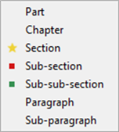
\includegraphics[scale=0.50]{./res/menu_insert_latex_header.png}\\

\begin{scriptsize}
  \begin{tabularx}{\textwidth}{>{\hsize=0.2\hsize}X>{\hsize=0.8\hsize}X}\\
    \hline
    \textbf{Option} & \textbf{Description} \\
    \hline
    Part & Inserts \textbf{$\backslash$part\{\}} if no selection or
     \textbf{$\backslash$part\{\texttt{selected}\}} \\
    Chapter & Inserts \textbf{$\backslash$chapter\{\}} if no selection or
     \textbf{$\backslash$chapter\{\texttt{selected}\}} \\
    Section & Inserts \textbf{$\backslash$section\{\}} if no selection or
     \textbf{$\backslash$section\{\texttt{selected}\}} \\
    Sub-section & Inserts \textbf{$\backslash$subsection\{\}} if no selection or
     \textbf{$\backslash$subsection\{\texttt{selected}\}} \\
    Sub-sub-section & Inserts \textbf{$\backslash$subsubsection\{\}} if no selection or
     \textbf{$\backslash$subsubsection\{\texttt{selected}\}} \\
    Paragraph & Inserts \textbf{$\backslash$paragraph\{\}} if no selection or
     \textbf{$\backslash$paragraph\{\texttt{selected}\}} \\
    Sub-paragraph & Inserts \textbf{$\backslash$subparagraph\{\}} if no selection or
     \textbf{$\backslash$subparagraph\{\texttt{selected}\}} \\
    \hline
  \end{tabularx}
\end{scriptsize}


\hypertarget{menu_insert_latex_format}{}
\subsubsection{Format:}\\
\index{insert menu!LaTeX format}

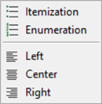
\includegraphics[scale=0.50]{./res/menu_insert_latex_format.png}\\

\begin{scriptsize}
  \begin{tabularx}{\textwidth}{>{\hsize=0.2\hsize}X>{\hsize=0.8\hsize}X}\\
    \hline
    \textbf{Option} & \textbf{Description} \\
    \hline
    Itemization & Inserts itemization or itemizes a selection \\
    Enumeration & Inserts enumeration or enumerates a selection \\
    \hdashline[1pt/1pt]
    Left & Inserts tag to align the text on the left or to align the selection on the left \\
    Center & Inserts tag to align the text on the center or to centralize the selection \\
    Right & Inserts tag to align the text right or to align the selection on the right \\
    \hline
  \end{tabularx}
\end{scriptsize}


\newpage
\hypertarget{menu_insert_latex_font}{}
\subsubsection{Font:}\\
\index{insert menu!LaTeX font}

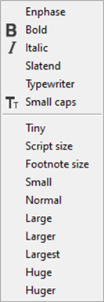
\includegraphics[scale=0.50]{./res/menu_insert_latex_font.png}\\

\begin{scriptsize}
  \begin{tabularx}{\textwidth}{>{\hsize=0.2\hsize}X>{\hsize=0.8\hsize}X}\\
    \hline
    \textbf{Option} & \textbf{Description} \\
    \hline
    Enphase & Inserts \textbf{$\backslash$emph\{\}} if no selection or
     \textbf{$\backslash$emph\{\texttt{selected}\}} \\
    Bold & Inserts \textbf{$\backslash$textbf\{\}} if no selection or
     \textbf{$\backslash$textbf\{\texttt{selected}\}} \\
    Italic & Inserts \textbf{$\backslash$textit\{\}} if no selection or
     \textbf{$\backslash$textit\{\texttt{selected}\}} \\
    Slatend & Inserts \textbf{$\backslash$textsl\{\}} if no selection or
     \textbf{$\backslash$textsl\{\texttt{selected}\}} \\
    Typewriter & Inserts \textbf{$\backslash$texttt\{\}} if no selection or
     \textbf{$\backslash$texttt\{\texttt{selected}\}} \\
    Small caps & Inserts \textbf{$\backslash$textsc\{\}} if no selection or
     \textbf{$\backslash$textsc\{\texttt{selected}\}} \\
    \hdashline[1pt/1pt]
    Tiny & Inserts \textbf{\{$\backslash$tiny \{\}\}} if no selection or
     \textbf{\{$\backslash$tiny \{\texttt{selected}\}\}} \\
    Script size & Inserts \textbf{\{$\backslash$scriptsize \{\}\}} if no selection or
     \textbf{\{$\backslash$scriptsize \{\texttt{selected}\}\}} \\
    Footnote size & Inserts \textbf{\{$\backslash$footnotesize \{\}\}} if no selection or
     \textbf{\{$\backslash$footnotesize \{\texttt{selected}\}\}} \\
    Small & Inserts \textbf{\{$\backslash$small \{\}\}} if no selection or
     \{$\backslash$small \textbf{\{\texttt{selected}\}\}} \\
    Normal & Inserts \textbf{\{$\backslash$normalsize \{\}\}} if no selection or
     \textbf{\{$\backslash$normalsize \{\texttt{selected}\}\}} \\
    Large & Inserts \textbf{\{$\backslash$large \{\}\}} if no selection or
     \textbf{\{$\backslash$large \{\texttt{selected}\}\}} \\
    Larger & Inserts \textbf{\{$\backslash$Large \{\}\}} if no selection or
     \textbf{\{$\backslash$Large \{\texttt{selected}\}\}} \\
    Largest & Inserts \textbf{\{$\backslash$LARGE \{\}\}} if no selection or
     \textbf{\{$\backslash$LARGE \{\texttt{selected}\}\}} \\
    Huge & Inserts \textbf{\{$\backslash$huge \{\}\}} if no selection or
     \textbf{\{$\backslash$huge \{\texttt{selected}\}\}} \\
    Huger & Inserts \textbf{\{$\backslash$Huge \{\}\}} if no selection or
     \textbf{\{$\backslash$Huge \{\texttt{selected}\}\}} \\
    \hline
  \end{tabularx}
\end{scriptsize}
